% !TEX TS-program = pdflatex
% !TEX encoding = UTF-8 Unicode

\documentclass{beamer}
%\documentclass[12pt,handout]{beamer}

\mode<presentation>{
	\usetheme{Singapore}
	% or ...

	\setbeamercovered{transparent}
	% or whatever (possibly just delete it)
}

\usepackage[english]{babel}
\usepackage{calc}
\usepackage[utf8]{inputenc}

\usepackage{kpfonts}
\usepackage[T1]{fontenc}

%\title[Building a Theremin] % (optional, use only with long paper titles)
%{Building a Theremin}

\title[Theremin\hspace{2em}\insertframenumber/
\inserttotalframenumber]{Building a Theremin}


\author[Wainwright] % (optional, use only with lots of authors)
{J.~Wainwright}
% - Use the \inst{?} command only if the authors have different
%   affiliation.

\institute[Universities of Somewhere and Elsewhere] % (optional, but mostly needed)
{
  Department of Physics and Astronomy\\
  University of Birmingham}
% - Use the \inst command only if there are several affiliations.
% - Keep it simple, no one is interested in your street address.

\date[Short Occasion] % (optional)
{24th Feb 2012}

\subject{J. Wainwright - Interview 24-02-12}
% This is only inserted into the PDF information catalog. Can be left
% out. 


% If you have a file called "university-logo-filename.xxx", where xxx
% is a graphic format that can be processed by latex or pdflatex,
% resp., then you can add a logo as follows:

% \pgfdeclareimage[height=0.5cm]{university-logo}{university-logo-filename}
% \logo{\pgfuseimage{university-logo}}

% Delete this, if you do not want the table of contents to pop up at
% the beginning of each subsection:
\AtBeginSubsection[]
{
  \begin{frame}<beamer>{Outline}
    \tableofcontents[currentsection,currentsubsection]
  \end{frame}
}


% If you wish to uncover everything in a step-wise fashion, uncomment
% the following command: 

\beamerdefaultoverlayspecification{<+->}

\setbeamertemplate{navigation symbols}{} 
\setbeamertemplate{footline}{\hspace*{.5cm}\scriptsize{\insertauthor 
\hspace*{50pt} \hfill\insertframenumber\hspace*{.5cm}}} 

\begin{document}

\begin{frame}
	\titlepage
\end{frame}

{
\usebackgroundtemplate{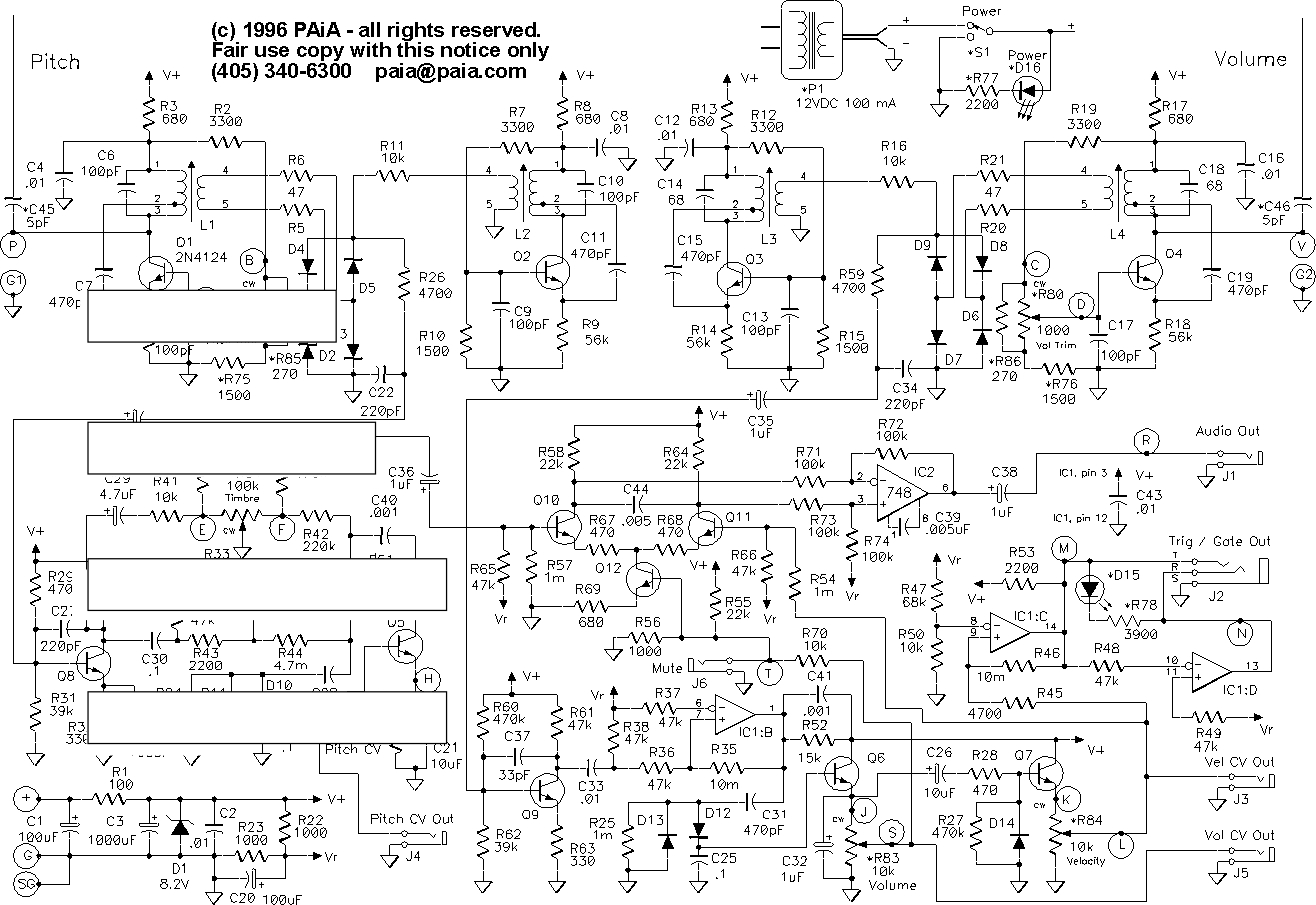
\includegraphics[width=\paperwidth]{Theremin/circuit_big2}}
\begin{frame}{Outline}
	\tableofcontents%[pausesections]
\end{frame}
}

\section{Introduction}

\begin{frame}{Task}
	\begin{itemize}
		\item As part of 2nd year Physics labs we had to choose a project to implement over a period of 11 weeks.
		\item Working in teams of 2 students
		\item The project that I chose was to "Build a Theremin"
	\end{itemize}
\end{frame}

\begin{frame}{Implementation}
First steps included;
	\begin{itemize}
		\item Research
		\begin{itemize}
			\item Complex circuits in commercial theremin
		\end{itemize}
		\item First ideas
		\item Concept designs
		\begin{itemize}
			\item Started from scratch
			\item Modular design to allow testing separately
		\end{itemize}
		\item Ordering parts
	\end{itemize} 
\end{frame}

\begin{frame}{History}
	\begin{itemize}
		\item Developed by Leon Termen, known in Europe as Leon Theremin.
		\item Invented in October 1920.
		\item By product of proximity sensor development.
		\item Shown to Lenin who dismissed it's usefulness but enjoyed the sound.
		\item Toured Europe to showcase the height of Russian technology.
	\end{itemize}
\end{frame}

\section{Basic Concept}

\begin{frame}{Basic Concept}
	\begin{columns}[c]
	\column{.8\textwidth}
		\begin{itemize}
			\item One of the only instruments you don't touch to play.
			\item Use two hands to interact with the instrument;
			\begin{itemize}
				\item One hand to control pitch.
				\item One hand to control volume.
			\end{itemize}
			\item The signals are produced by voltage control oscillators (VCOs).
		\end{itemize}
		\vspace{2cm}
	\column{.2\textwidth}
		\hspace{-5cm}
		\begin{centering}
			\pgfimage[width=0.5\paperwidth]{Theremin/theremin_pic}
			\par
		\end{centering}
	\end{columns}
\end{frame}

\begin{frame}{Basic Theory}
The electronics for each hand;
\begin{itemize}
	\item Involves 2 VCOs
		\begin{itemize}
			\item 1 as a control, remains fixed.	
			\item 1 is varied by the user
		\end{itemize}
	\item 2 signals added and subtracted by a mixer circuit to produce final signal.
\end{itemize}
\end{frame}

\begin{frame}{Signal Generator}
	\begin{itemize}
		\item As proof of concept, use a signal generator to output sinusoidal waveform.
		\item Send this wave through control method then to speaker to test.
		\item Can vary between sinusoidal, triangle and square waves.
		\item Test mixer when using two signals from the generator. 
	\end{itemize}
\end{frame}

\begin{frame}{Parallel Plate Capacitor}
	\begin{itemize}
		\item User acts as a grounded plate of parallel plate capacitor.
		\item Moving closer decreases the capacitance.
		\item When further away, the capacitance increases.
		\item Can make rough estimate of capacitance from the following capacitor equation;  
	\end{itemize}
\end{frame}

\begin{frame}{Capacitor Equation}
	\[
		C = \frac{k\varepsilon_0 A}{d}
	\]
	where 
	\begin{itemize}
		\pause \item $k = $ relative permeability of the dielectric material between the plates, in this case air =1,
		\item $\varepsilon_0 = $ permittivity of free space $= 8.854\times 10^{-12}Fm^{-1}$,
		\item $A = $ area of the plates,
		\item $d = $ separation of the plates, in this case the distance from the plate to the user's hand.
	\end{itemize}
\visible<6-> {Value estimated at $1.33\times 10^{-12}$F.}
\end{frame}

\section{Components Used}

\begin{frame}{555 Timer Chip}
	\begin{itemize}
		\item The 555 timer IC outputs a square wave with frequency depending on the input voltage.
		\item Can be used as a VCO, changing the resistances changes the input voltage - voltage divider theorem.
		\item Characteristics of produced wave controlled by the equations;
		\begin{align*}
			\text{Frequency, }f &= \frac{1}{\ln(2)C(R_1+R_2)} \\
			\text{Low time, }\tau_l &= \ln(2)R_2C \\
			\text{High time, }\tau_h &= \ln(2)(R_1+R_2)C
		\end{align*}
	\end{itemize}
\end{frame}

\begin{frame}{High Frequency}
	\begin{centering}
		\pgfimage[width=0.8\paperwidth]{Theremin/high_frequency}
		\par
	\end{centering}
\end{frame}

\begin{frame}{Low Frequency}
	\begin{centering}
		\pgfimage[width=0.8\paperwidth]{Theremin/low_frequency}
		\par
	\end{centering}
\end{frame}

%\begin{frame}{4046 VCO}
%	\begin{itemize}
%		\item CMOS Chip
%		\item Includes 2 phase comparators, a zener diode, but most importantly a Voltage Controlled Oscillator
%
%		\visible<3->{
%		\begin{centering}
%			\pgfimage[width=0.6\paperwidth]{Theremin/4046}
%			\par
%		\end{centering}}
%	\end{itemize}
%\end{frame}

\begin{frame}{Mixer Circuit}
The SA612A mixer chip is used for the mixer circuit.
	\begin{itemize}
		\pause \item Takes 2 input signals and outputs both the addition and subtraction of them.
		\item Contains internal oscillator, but not used for this purpose.
	\end{itemize}
	
	\visible<4->{
	\begin{centering}
		\pgfimage[width=0.5\paperwidth]{Theremin/SA612A}
		\par
	\end{centering}}
\end{frame}

\begin{frame}{Mixer Signal}
	\vspace{-2cm}\begin{centering}
		\pgfimage[width=0.9\paperwidth]{Theremin/mixer_out1}
		\par
	\end{centering}
	\vspace{-4.cm}\begin{centering}
		\pgfimage[width=0.9\paperwidth]{Theremin/low_pass_filter1}
		\par
	\end{centering}
\end{frame}

\section{Testing}

\begin{frame}{Low Pass Filter}
\emph{Low pass filter} - electronic filter that passes low-frequency signals but reduces the amplitude of signals with frequencies higher than the cutoff frequency.
	\begin{columns}[c]
		\column{.7\textwidth}
		\begin{itemize}
			\item Use to remove the high frequency oscillations in waveform
			\item Consists of simple cheap components;
			\begin{itemize}
				\item Resistors
				\item Capacitor
				\item Op-amp
			\end{itemize}
			\item When arranged in the right way will give large control over frequencies blocked.
		\end{itemize}
		\column{.3\textwidth}
		\visible<2->{
		\hspace{-2.5cm}\begin{centering}
			\pgfimage[width=0.4\paperwidth]{Theremin/Active_Lowpass_Filter_RC}
			\par
		\end{centering}}
	\end{columns}
\end{frame}

\begin{frame}{Progress}
	\begin{centering}
		\pgfimage[width=0.7\paperwidth]{Theremin/Photo0089}
		\par
	\end{centering}
\end{frame}

\begin{frame}{Progress}
	\begin{centering}
		\pgfimage[width=0.7\paperwidth]{Theremin/Photo0078}
		\par
	\end{centering}
\end{frame}

\begin{frame}{Progress}
	\begin{centering}
		\pgfimage[width=0.7\paperwidth]{Theremin/Photo0087}
		\par
	\end{centering}
\end{frame}

\begin{frame}{Progress}
	\begin{centering}
		\pgfimage[width=0.7\paperwidth]{Theremin/Photo0088}
		\par
	\end{centering} 
\end{frame}

\begin{frame}{Progress}
	\vspace{-1cm}
	\begin{centering}
		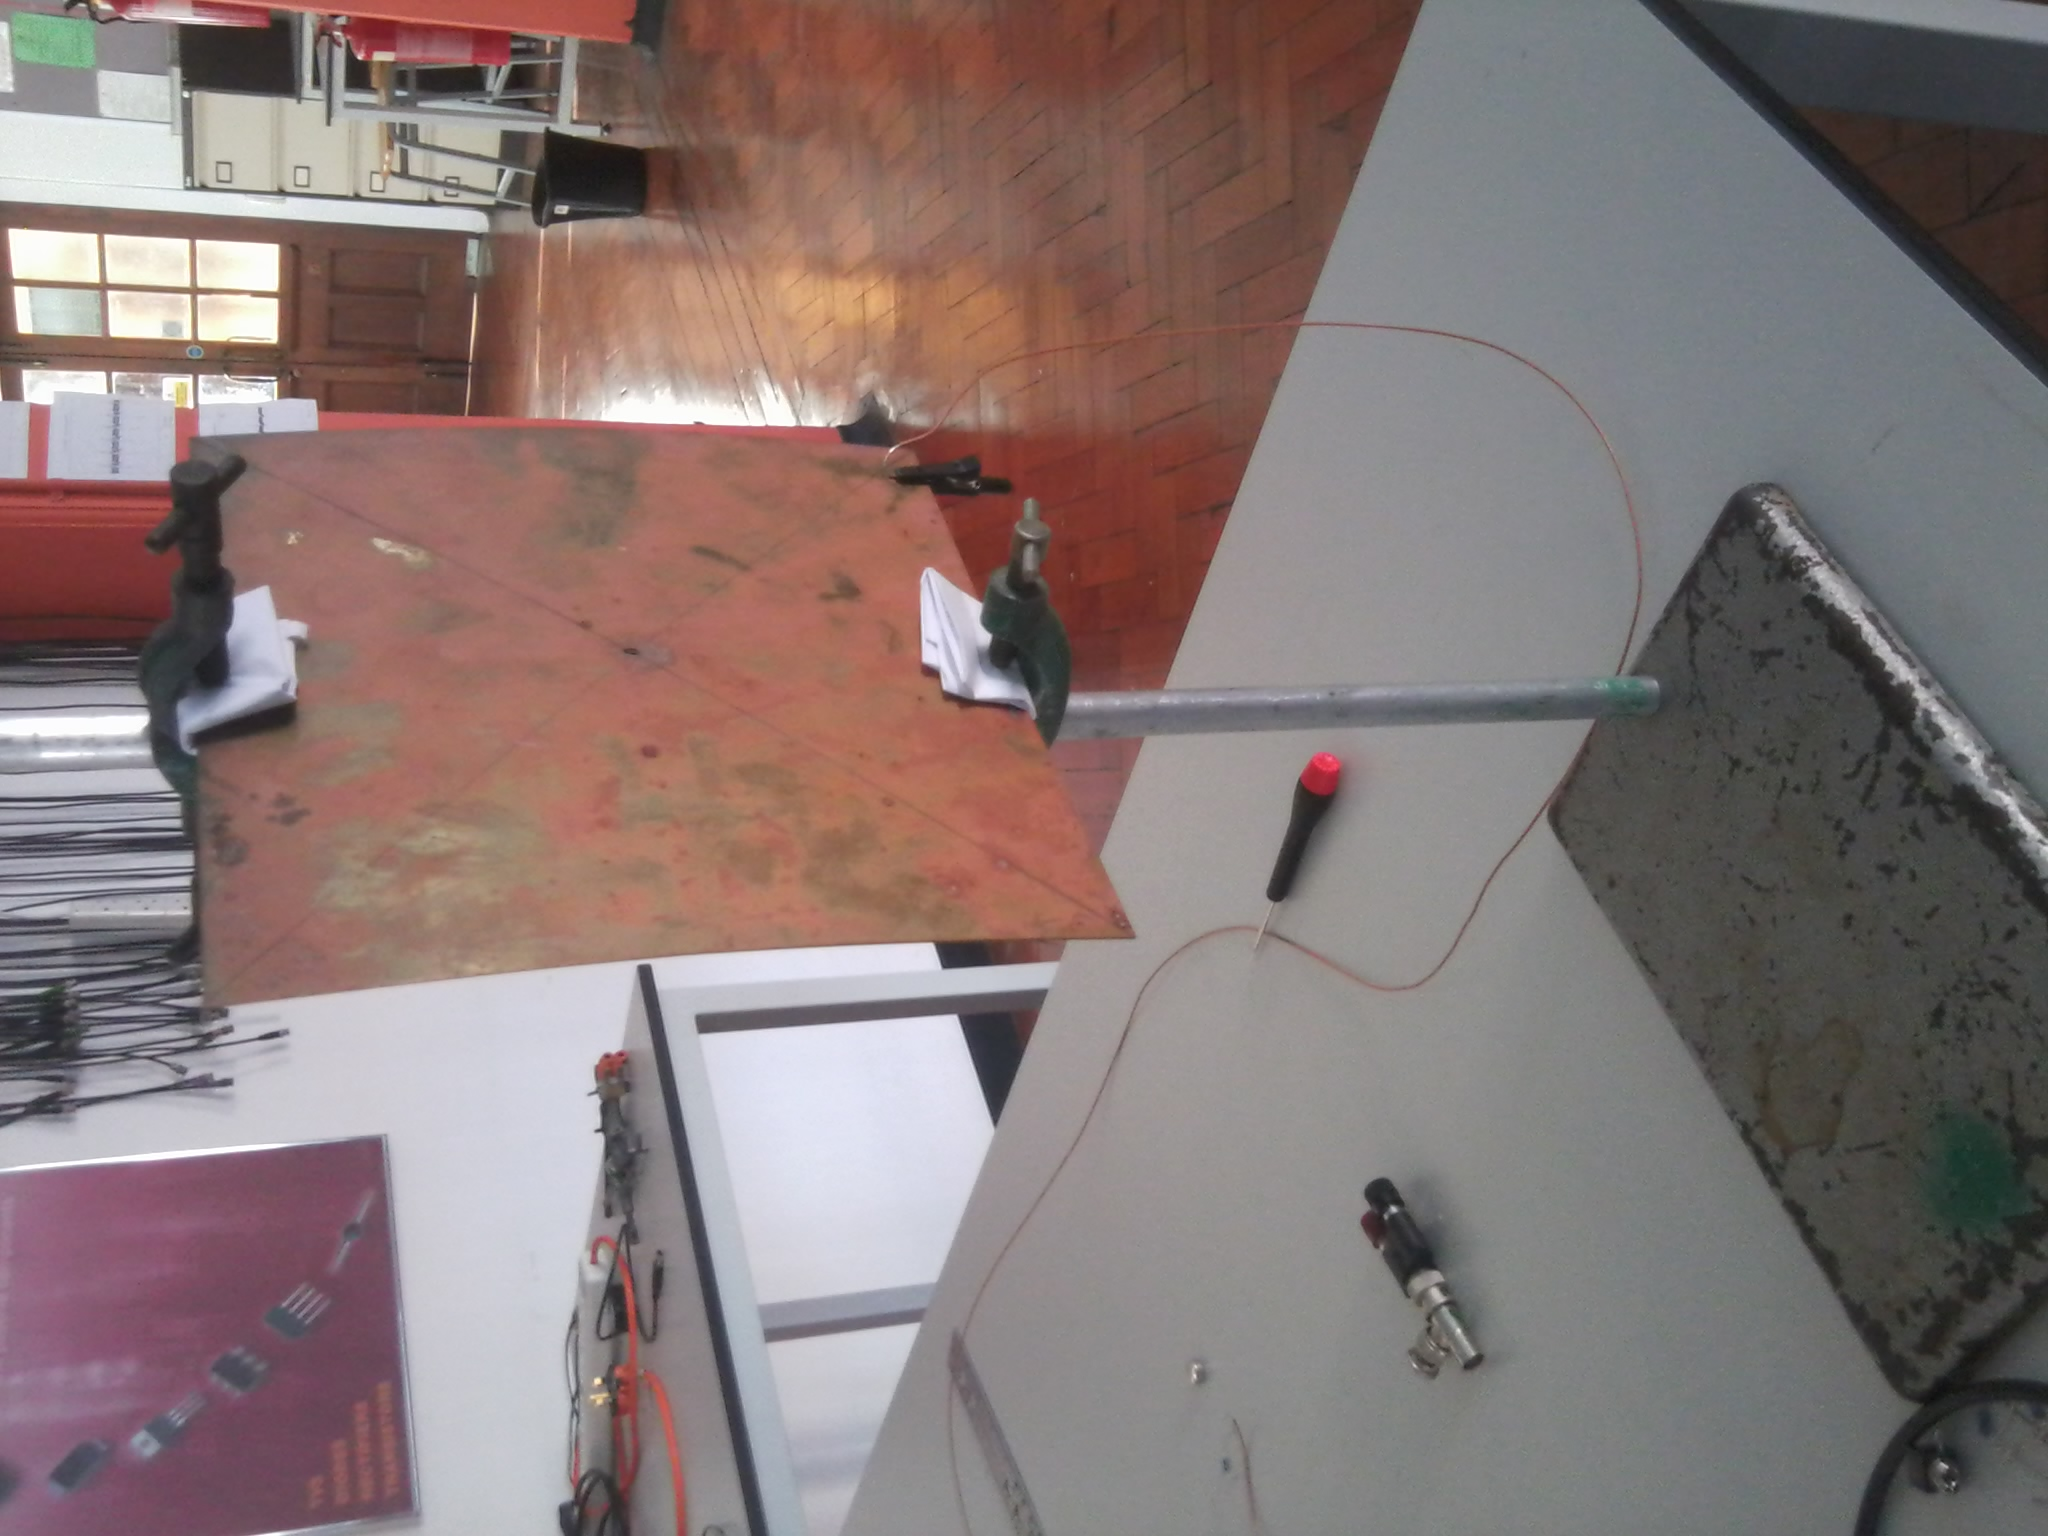
\includegraphics[angle=270, width=0.51\paperwidth]{Theremin/Photo0090}
		%[width=0.7\paperwidth]{Theremin/Photo0090}
		\par
	\end{centering} 
\end{frame}

\section*{Summary}

\begin{frame}{Summary}
	\begin{itemize}
		\item Building a \alert{theremin} in 11 weeks from scratch.
		\item Using \alert{commonly available} components and resources.
	\end{itemize}
	\vskip0pt plus.5fill
	\begin{itemize}
		\item Outlook
		\begin{itemize}
			\item Testing to improve quality and performance.
			\item Reduce size and power requirements for commercialisation.
		\end{itemize}
	\end{itemize}
\end{frame}

\end{document}


